\documentclass[12pt,a4paper]{article}
\usepackage[utf8]{inputenc}
\usepackage{fancyhdr}
\usepackage{datetime2}
\usepackage{parskip}
\usepackage{spverbatim}
\usepackage{graphicx}
\usepackage{float}
\usepackage{listings}
\usepackage{xcolor}
\usepackage{amsmath}
% \graphicspath{{plots/}}
% \newcommand{\imgw}{0.8}

\pagestyle{fancy}
\fancyhf{}

\lhead{TDDE16}
\rhead{\today} % yyyy-mm-dd
\setlength{\headheight}{15pt}

\cfoot{\thepage}

\begin{document}

\begin{center}
    \Huge
    \textbf{Dota mining}

    \vspace{0.3cm}
    \large
    Ludvig Noring \
    ludno249

\end{center}

\section{Introduction}
From my personal experience of the competitive online gaming culture
people tend to be expressive in what ever means of communication available to them.
A win is much more enjoyed if you can rub it in the opponents face.
A individual mistake can be mitigated if you put the blame on your teammates.

I am interested in creating a classifier to predict the outcome of a match and how different features perform,
by only looking only at the chat from games of Dota 2.

Dota 2 is an online multiplayer game where ten players are divided into two teams
with the objective to destroy the opposing team's base.
To achieve this all five players within a team depend on each others performance.
The teams can communicate with each other using the in-game chat.

\section{Theory}
In this section theory about the classifier and the features used will be presented.

\subsection{Naive Bayes}
The Naive Bayes classifier will assign the most probable class given a feature vector.
Bayesian classifiers in general all work this way but what puts the naive in naive bayes
is that it assumes all features are independent of each other.
This naive approach simplifies learning while still maintaining performance.\cite{bayes}

When training the classifier a set of features need to be decided on.
Since the same feature vector need to be used for all documents some preprocessing of the corpus
might be needed.
Then using this set of features a feature vector for each document in the training set is
computed and fed to the classifier.
Training the model falls under supervised learning so the correct class is needed together with the feature vector.
With this information the classifier can calculate the probability for each class and the probability for each feature given a class.

When the model is trained a new document can be introduced for classification.
The document is parsed and features are extracted in the same way as in the training phase.
The most probable class is the calculated by using the formula below where $C$ is the class, win or lose
and $x$ is the feature vector.

$$\hat{y} = \underset{k \in \{1,2,...,K\}}{argmax} \, \, \, p(C_{k}) \prod_{i=1}^{n} p (x_{i}|C_{k})$$

\subsection{Shannon Diversity Index}
When investigating how diverse a data set is a diversity index can be used.
It is used as a measure of how many types or bins there are and how many there are in each bin.
For example looking at the grades of a school class the bins would be the different grades
and each student's grade would be placed in the appropriate bin.
If the students have very diverse grades the bins would be of similar size and the diversity index would be high.
If on the other hand a class was too difficult and many of the students failed the \textit{fail bin} would fill up
and the diversity index would decrease.
The index is calculated using the formula below where R is the number of bins. The index ranges from $0$ to $\ln{R}$.
$$H' = -\sum_{i=1}^{R}p_i \ln{p_i}$$

\subsection{N-grams}
An n-gram is a set of words or letters of length n.
They can be used for various applications such as language models for predicting following words letters.
N-grams of length one is referred to as unigrams, length of two bigrams and length of three trigrams.

\section{Method}
The system was built by first collecting data to create a corpus.
Then a classifier was be built and trained using the created corpus.
Different features were used and evaluated.

\subsection{Collecting data}
The first step towards creating our classifier is establishing a data set containing chat logs from thousands of matches.
\textit{opendota.com} offers a free api for collecting various data about Dota 2 matches.
The api was queried to return matches only in the above average skill level.
This was to eliminate all practice matches against bots containing no chat,
and also to make sure the players playing are familiar to the terminology of Dota.
Matches were nothing was written was discarded.
No threshold was decided on creating the data set so matches containing only a single word was included.
The filtering was done later when training the classifier.

The chat logs could only be retrieved from the api one match at a time.
This resulted in a slow gathering of chat logs.
In response to this the corpus was built successively.

\subsection{Naive Bayes Classifier}
The classifier was implemented using the Python library \textit{nltk}.
The library provides a generic Naive Bayes classifier complete with training and classifying methods.

The classifier was extended with functionality to parse the corpus.
Matches were both teams did not write five words or more were discarded.
The chat log was extracted together with information about what player said what,
match duration and the match winner.
Half of the corpus was used for training and the other half was used for testing.

\subsubsection{Features}
\label{sec:feats}
After the corpus has been parsed it was be processed further to extract all unigrams, bigrams and trigrams.
The messages of all players within a team were chronologically concatenated to a single document.
Many n-grams are only occurring once throughout the corpus.
This might be because of spelling or simply because the words or phrases are rarely used.
These n-grams were considered irrelevant and discarded to decrease training time without affecting performance.
When the classifier had built its vocabulary it could featurize all matches in the training set.
The features used for the classifier are:
\begin{itemize}
    \item Unigrams
    \item Bigrams
    \item Trigrams
    \item Words per 30 minutes (a game of Dota usually last around 30 minutes)
    \item Shannon Diversity Index
\end{itemize}
The feature vector for each match contains boolean values for all features. All n-grams are an individual feature.
If a chat log contains an n-gram seen in training that n-gram would get the boolean value True and if not False.
Wp30 was digitized to $5$ values linearly distributed between $0$ and $200$
and sdi was digitized to $5$ values linearly distributed between $0$ and $\ln{5}$.

\subsubsection{Testing}
When evaluating the performance of the classifier worked logically very similar as the training phase.
The testing set was first parsed in the same way as in training.
Then each document could be featurized and fed into the classifier resulting in a probability for victory.
Since each match has one winner and one loser the classifier can either try and predict each team's chat log individually
or it can decide which of the two teams is the most probable winner.
In this project both methods were used and evaluated.

\subsection{Baseline System}
A baseline system was created using the whole data set split up into 50\% training and 50\% testing.
When training the baseline classifier the features were limited to only unigrams.
The unigrams were extracted and trained upon in the same way as described in \ref{sec:feats}.

\section{Result}
In the later stages of the project the corpus contained a total of 3946 matches.
The number of n-grams extracted from the training set i.e. half of the matches,
can be seen in table \ref{tab:n-grams}

\begin{table}[h]
    \begin{center}
        \begin{tabular}{r | c c}
                        & Total & $>1$   \\
            \hline
            Unigrams    & 18940 & 6173 \\
            Bigrams     & 75703 & 8852 \\
            Trigrams    & 94083 & 2097 \\
        \end{tabular}
        \caption{N-gram frequency}
        \label{tab:n-grams}
    \end{center}
\end{table}

The words per 30 minutes and Shannon diversity index features both need to be digitized
to help the classifier. The Shannon diversity index bins were decided upon by simple
trial and error. The wp30 bins took help from how the data was distributed.
The histogram of wp30 can be seen in figure \ref{fig:wp30}.
\begin{figure}[h]
    \centering
    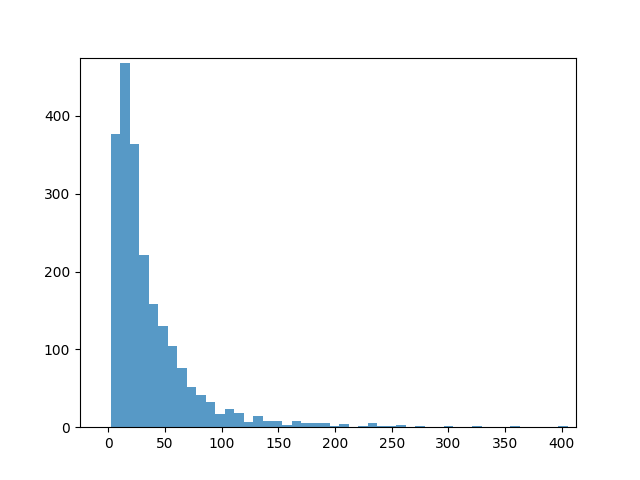
\includegraphics[width=0.8\textwidth]{wp30.png}
    \caption{wp30 distribution}
    \label{fig:wp30}
\end{figure}

\subsection{Baseline System}
The baseline system trained on 2178 matches using only unigrams with a frequency greater than one.
The performance of the baseline system can be seen in table \ref{tab:baseline}.
Precision and recall has been calculated for both outcomes.
Both the accuracy for classifying individual chat logs and the accuracy for
classifying the match winner is shown.

\begin{table}[h]
    \begin{center}
\begin{tabular}{ r | l l }
                & Win       & Lose \\
    \hline
    Precision   & 57.27\%   & 64.47\% \\
    Recall      & 76.25\%   & 43.10\% \\
    % F-Measure   & 64.89\%   & 52.45\% \\
    %\hline
    
\end{tabular}

\rule{0pt}{8ex}    
\begin{tabular}{ l l }
    Individual accuracy: & 59.67\% \\
    Per match accuracy:  & 68.10\%\\
\end{tabular}
\caption{Baseline performance}
\label{tab:baseline}
\end{center}
\end{table}

The most informative unigrams of the baseline system is presented in table \ref{tab:unigrams}.
The italicized words in the table are in russian. 
\begin{table}[h]
    \begin{center}
        \begin{tabular}{l | c}
            Unigram    & Ratio (win:lose) \\\hline
            throne            & 1.0 : 13.0 \\
            \textit{midu}     & 1.0 : 10.3 \\
            \textit{bozhe}       & 1.0 : 6.3 \\
            picked    & 1.0 : 6.3 \\
            cumback   & 6.3 : 1.0 \\
            jebaited          & 5.9 : 1.0 \\
            moron           & 1.0 : 5.7 \\
            crying                & 1.0 : 5.7 \\
            3k           & 1.0 : 5.3\\
            hand            & 1.0 : 5.0 \\
            intro   & 5.0 : 1.0 \\
        \end{tabular}
        \caption{Baseline's most informative features}
        \label{tab:unigrams}
    \end{center}
\end{table}

\subsection{Individual Features}
The features used in this project were all evaluated individually using the same method as with the baseline system.
In table \ref{tab:featpref} both the individual chat log accuracy and the per match accuracy is presented
for the features.

\begin{table}[h]
    \begin{center}
        \begin{tabular}{ r | l l l l }
                                  & Bigram  & Trigram & wp30    & sdi \\ \hline
            Individual accuracy   & 62.93\% & 54.26\% & 51.05\% & 54.17\% \\
            Per match accuracy    & 70.31\% & 38.31\% & 13.89\% & 39.08\% \\
        \end{tabular}
        \caption{Individual feature performance}
        \label{tab:featpref}
    \end{center}
\end{table}

The ten most informative features when training on bigrams and trigrams individually can be
seen in table \ref{tab:ngrams}.
\begin{table}[h]
    \begin{center}
        \begin{tabular}{l | c | l | c}
            Bigram     & Ratio (win:lose) & Trigram & Ratio (win:lose) \\\hline
            commend me & 12.6 : 1.0 & e ez ez        & 7.0 : 1.0 \\
            gg commend & 9.7 : 1.0  & haha haha haha & 5.6 : 1.0 \\
            hahaha why & 9.0 : 1.0  & ez mid haha    & 5.0 : 1.0 \\
            me report  & 1.0 : 8.6  & ez game ez     & 5.0 : 1.0 \\
            haha commend  & 8.3 : 1.0  & hahaha hahahaha hahaha     & 4.3 : 1.0 \\
            es report  & 1.0 : 8.3  & haha ez ez     & 4.3 : 1.0 \\
            hahah ez  & 7.7 : .10  & haha hahaha hahaha     & 4.2 : 1.0 \\
            just end  & 1.0 : 7.6  & let us end     & 4.2 : 1.0 \\
            me ez  & 7.3 : 1.0  & z ez ez     & 3.9 : 1.0 \\
            he did  & 1.0 : 7.0  & ez ez e     & 3.9 : 1.0 \\

        \end{tabular}
        \caption{Bigram \& trigram informative features}
        \label{tab:ngrams}
    \end{center}
\end{table}

The most informative features when training on words per 30 minutes and Shannon diversity index
individually can be seen in table \ref{tab:sdi}.

\begin{table}[h]
    \begin{center}
        \begin{tabular}{l | c | l | c}
            wp30     & Ratio (win:lose) & sdi & Ratio (win:lose) \\\hline
            $150<200$  & 1.0 : 2.4  & $1.21<1.61$    & 1.6 : 1.0 \\
            $>=200$  & 1.0 : 1.7  & $0<0.40$   & 1.0 : 1.6 \\
            $100<150$ & 1.0 : 1.5  & $0.40<0.80$  & 1.0 : 1.1 \\
            $50<100$ & 1.1 : 1.0  &  $0.80<1.21$  & 1.1 : 1.0 \\
            $0<50$ & 1.0 : 1.0 & &  \\

        \end{tabular}
        \caption{Bigram \& trigram informative features}
        \label{tab:sdi}
    \end{center}
\end{table}

\subsection{Complete System}
Combining all the features, still training on the same training set as in the previous section,
resulted in performance presented in table \ref{tab:complete}.


\begin{table}[h]
    \begin{center}
\begin{tabular}{ r | l l }
                & Win       & Lose \\
    \hline
    Precision   & 60.97\%   & 69.85\% \\
    Recall      & 78.54\%   & 49.71\% \\
    %F-Measure   & 68.65\%   & 58.09\% \\
    %\hline
    
\end{tabular}

\rule{0pt}{8ex}    
\begin{tabular}{ l l }
    Individual accuracy: & 64.13\% \\
    Per match accuracy:  & 74.52\%\\
\end{tabular}
\caption{Complete system performance}
\label{tab:complete}
\end{center}
\end{table}

The most informative features of the complete system is presented in table \ref{tab:completefeats}.
\begin{table}[h]
    \begin{center}
        \begin{tabular}{l | c}
            Feature          & Ratio (win:lose) \\ \hline
            throne           & 1.0 : 13.0 \\
            commend me       & 12.6 : 1.0 \\
            \textit{midu}    & 1.0 : 10.3 \\
            gg commend       & 9.7 : 1.0 \\
            hahaha why       & 9.0 : 1.0 \\
            me report        & 1.0 : 8.6 \\
            haha commend     & 8.3 : 1.0 \\
            es report        & 1.0 : 8.3 \\
            hahah ez         & 7.7 : 1.0 \\
            just end         & 1.0 : 7.6 \\
        \end{tabular}
        \caption{Complete system's most informative features}
        \label{tab:completefeats}
    \end{center}
\end{table}

% \subsection{Using the System}


\section{Discussion}
The final size of the corpus used was close to 4000 matches.
Much earlier work by others has been done using the Naive Bayes classifier.
Ion Androutsopoulos et. al \cite{spam} has done a successful
spam filter using a corpus of size just under 2000 documents.
Bo Pang et. al \cite{sentiment} doing a sentiment analysis
using the naive bayes classifier used training and testing sets of 1000 each.

\subsection{Baseline System}
The measure in focus when evaluating the systems was accuracy. Since both classes, win or lose,
are both equally important.
The individual accuracy of the baseline system was $59.67\%$ and the per match accuracy was $68.10\%$.
The per match accuracy is significantly higher than the individual accuracy.
This is not very surprising.
A incorrect classification with low confidence can be \textit{saved} if the other team's chat log
is correctly classified with a higher confidence.

Two of the top most informative unigrams for the baseline system was in russian.
This is mainly because of the large number of russian people playing the game \cite{ruski}.
The highest of the two \textit{midu} meaning mid. 
\textit{me mid} or just \textit{mid} is a phrase used when you want to take the role as the
middle player. The middle player in Dota often has a high impact and can more often than not
decide the outcome of the game. Winning the game as a mid player can to many be more rewarding
knowing that you were a \textit{obvious} part of the victory. Compared to other role such as
the support player which have a much less obvious impact on the outcome.
A player using the chat to acquire the mid role might be more interested in personal gain
and less interested in the team effort and therefore less prone to teamwork.

The second russian word \textit{bozhe} is the equivalent for the interject \textit{god} or \textit{christ!}.
Commonly used to exclaim disappointment in your teammates.

The objective of the game is to destroy your opponents throne. The most informative unigram is throne.
This phrase is often used to ask your opponent to march directly towards your base and end the game.


% Individual feature accuracy
\subsection{Individual Features}
The performance for the features individually can be seen in table \ref{tab:featpref}.
Using bigrams the classifier performed better than the baseline looking at both the individual accuracy
and the per match accuracy.
The rest of the features performed worse than the unigram baseline.
wp30 being the least informative feature.
Why the per match accuracy is much lower than the individual accuracy is because when
doing the comparison between the two team's class probability, the classifier predicts the
wrong team if the probabilities are 50/50.
For example if both team fall in the same wp30 or sdi bin the classifier will get one correct
for the individual accuracy but both wrong in the per match accuracy.

% n-grams. Dirty data
\subsection{N-grams}
Looking at the n-grams presented in table \ref{tab:n-grams} some reoccurring phrases are the most informative.
After a match players can \textit{commend} each other as a compliment.
Players having performed well will more likely ask for such commendations.
It is therefore not very surprising nor interesting that the bigrams containing variation of this phrase
are a good indicator of victory.
Similarly players can report each other after each game which is basically the opposite of commending.

The n-grams were extracted by concatenating all the messages from a team.
Because of this the n-grams are not necessarily from the same chat message or even the same player.
This is clearly seen in the most informative trigrams.
The only trigram which is a single chat message is \textit{let us end} while the others are just
laughter or variations of \textit{ez} (short for easy).

The trigrams also show another \textit{flaw} with the corpus, that the language is very non formal and
could be cleaned up. Adding one extra \textit{ha} to your laughter should not be treated
as a completely different word.

\subsection{wp30 and sdi}
While both features wp30 and sdi performed much worse than the n-grams they still show some
interesting results.
Teams which write much and score low on the diversity index show some tendency to lose,
while teams which write less and score higher on the index are more a little more likely to win.


% Complete system accuracy and to feats
\subsection{Complete System}
Running the system with all features enabled resulted in the performance shown in table \ref{tab:complete}.
The accuracy achieved with the complete system outperformed both the baseline and all the feature's
individual performance.
Only unigrams and bigrams made it into the ten most informative features.

Both the baseline and the complete system performed better on predicting teams as winners.
Precision was slightly worse classifying winners but with a recall close to 80\% for both systems.

\section{Conclusion}
Using the opendota API to create a corpus of Dota 2 chat logs to train and test a naive bayes classifier
resulted in a decent performance.
Different features were evaluated and n-grams came out on top regarding performance.
The language used in Dota 2 is simple and short phrases are often used to convey the information necessary.
Unigrams and bigrams therefore suffice in length to cover whole phrases.
Because of this the n-grams are not very interesting from a language processing perspective.
The worse performing word rate and diversity index features show some promise and could maybe be improved
further.
One idea could be to use information about the opposing team when featurizing the documents.
Chatting is often a dialog between the two teams so the teams individual chat logs should be dependant
of each other.

The system can be used by cloning the GitHub repository and following the instructions from the Readme.
The final corpus used in the project is hosted in the repository.

\pagebreak
\bibliographystyle{ieeetr}
\bibliography{report}
\end{document}


